\section{Materiales y métodos}

\subsection{Materiales: datos generalistas}
\begin{frame}
    \frametitle{Materiales: datos generalistas (SJTU)}
    \begin{columns}
      \column{0.5\textwidth}
      \begin{enumerate}
        \item \textbf{10 nubes de puntos} de referencia.  
        \item \textbf{7} tipos de \textbf{distorsiones}: compresión, ruido al color, 
          ruido geométrico, ruido gaussiano y combinación entre ellas.
        \item \textbf{6 niveles} de intensidad.
        \item \textbf{Total de 420 nubes de puntos}.
      \end{enumerate}
      \column{0.5\textwidth}
      \begin{figure}
        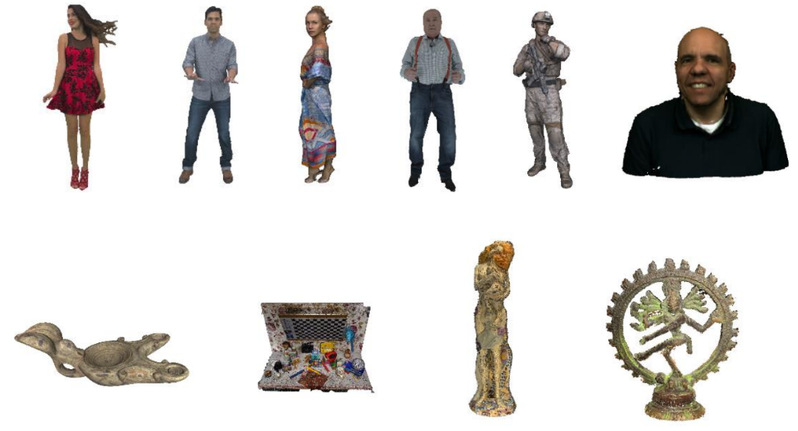
\includegraphics[width=0.95\textwidth]{imagenes/chapter3/SJTU}
        \caption{Ejemplo de conjuntos de datos SJTU\footnotemark}
        \label{fig:SJTU}
      \end{figure}
    \end{columns}
    \footcitetext{SJTU}
\end{frame}

\begin{frame}
    \frametitle{Materiales: datos generalistas (WPC)}
    \begin{columns}
      \column{0.5\textwidth}
      \begin{enumerate}
        \item \textbf{25 nubes de puntos} de referencia.  
        \item \textbf{5} tipos de \textbf{distorsiones}: 
          sumuestreo, ruido gaussiano, \emph{trisoup}, V-PCC y \emph{octree}.
        \item Longitud de \textbf{intensidades variantes}.
        \item \textbf{Total de 741 nubes de puntos}.
      \end{enumerate}
      \column{0.5\textwidth}
      \begin{figure}
        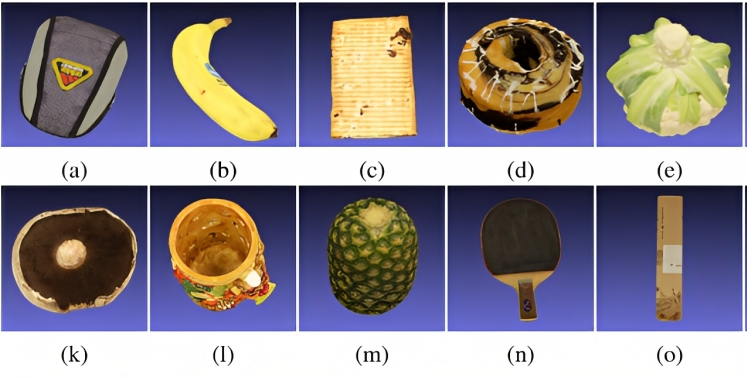
\includegraphics[width=.95\textwidth]{imagenes/chapter3/WPC}
        \caption{Ejemplo de conjuntos de datos WPC\footnotemark}
        \label{fig:WPC}
      \end{figure}
    \end{columns}
    \footcitetext{WPC1}
\end{frame}

\begin{frame}
  \frametitle{Materiales: datos generalistas (LS-PCQA)}
  \begin{columns}
    \column{0.5\textwidth}
    \begin{enumerate}
      \item \textbf{104 nubes de puntos} de referencia.  
      \item \textbf{31} tipos de \textbf{distorsiones}.
      \item \textbf{7 niveles} de intensidad.
      \item \textbf{Total de 22000 nubes de puntos}.
    \end{enumerate}
    \column{0.5\textwidth}
    \begin{figure}
      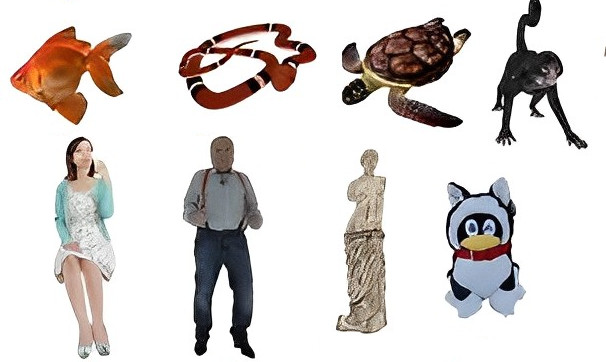
\includegraphics[width=0.8\textwidth]{imagenes/chapter3/LSPCQA}
      \caption{Ejemplo de conjuntos de datos LS-PCQA\footnotemark}
      \label{fig:LSSJTU}
    \end{figure}
  \end{columns}
  \footcitetext{ResSCNN}
\end{frame}

\subsection{Materiales: datos sintéticos}
\begin{frame}
  \frametitle{Materiales: datos sintéticos}
  \vspace{-.8cm}
    \begin{figure}[htp]
      \subfloat[]{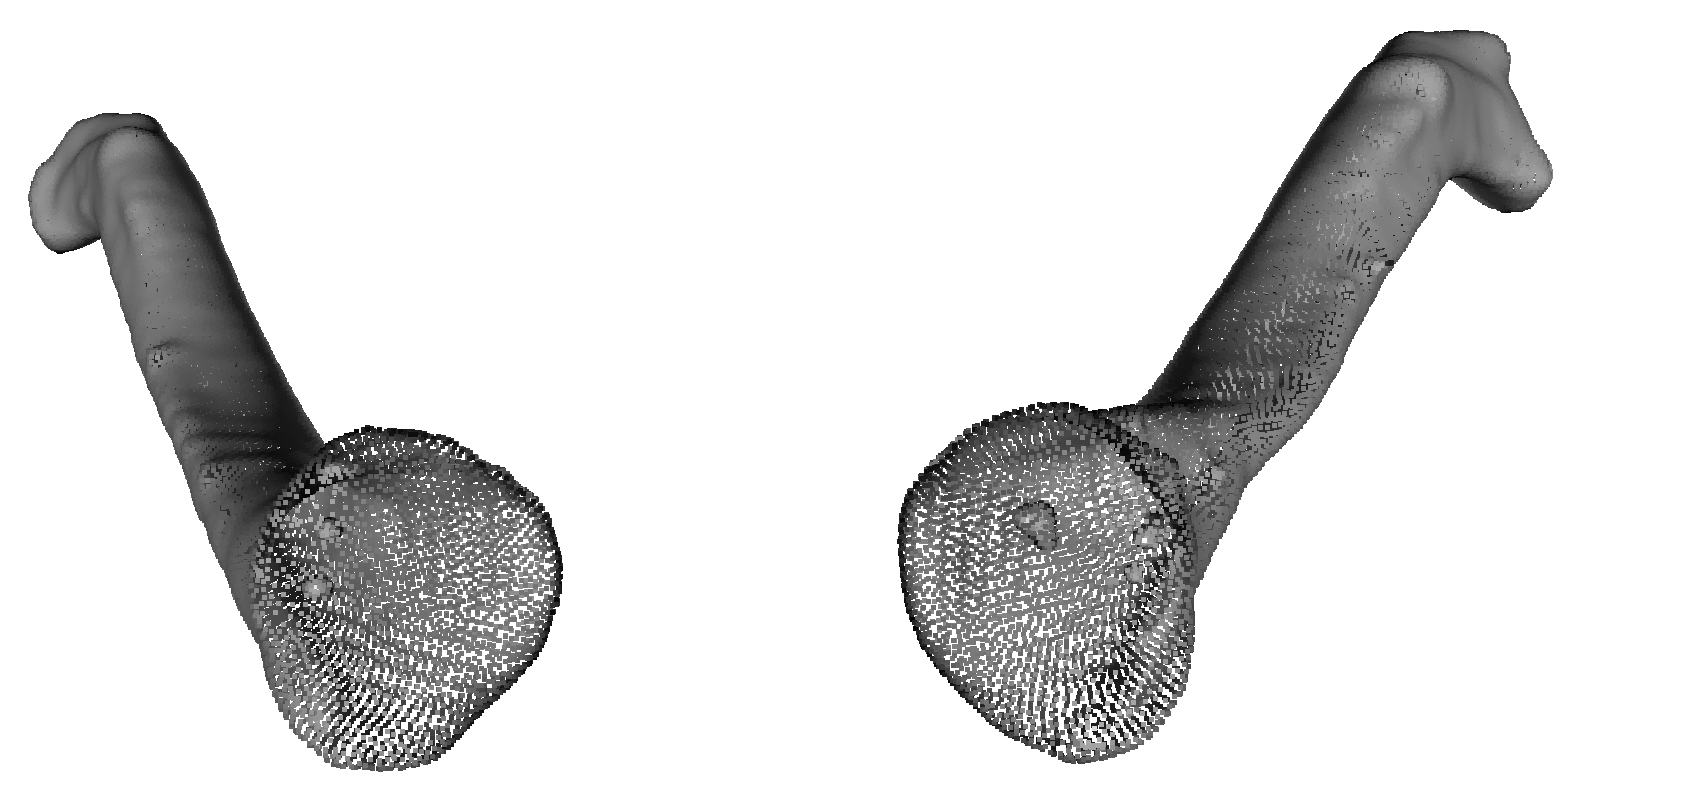
\includegraphics[width=.3\textwidth]{imagenes/chapter3/clavicula/clavicula_0.png}}
      \subfloat[]{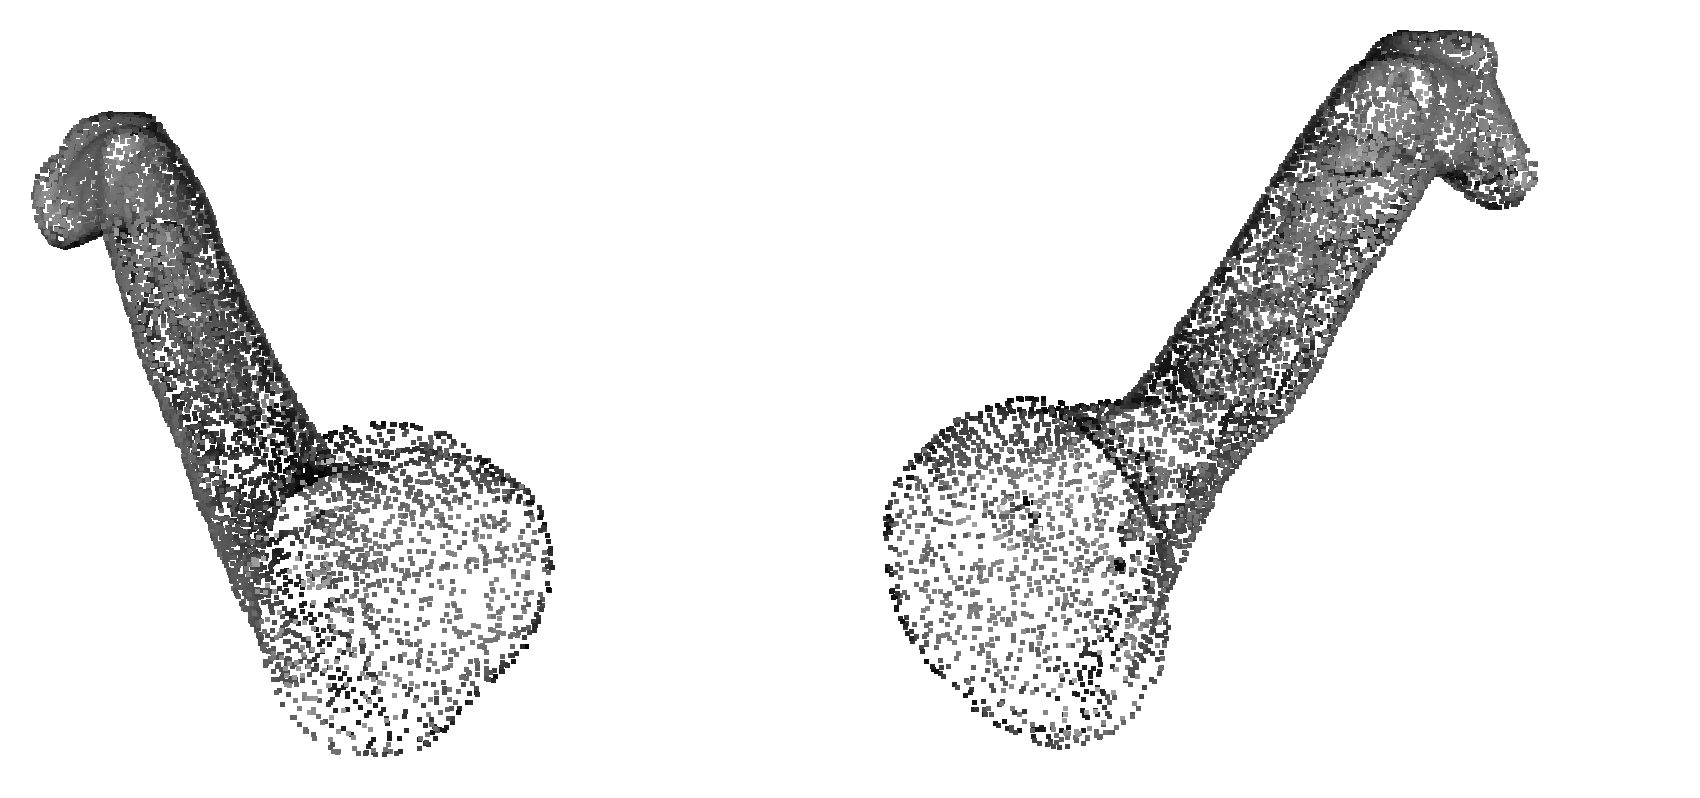
\includegraphics[width=.3\textwidth]{imagenes/chapter3/clavicula/clavicula_2.png}}
      \subfloat[]{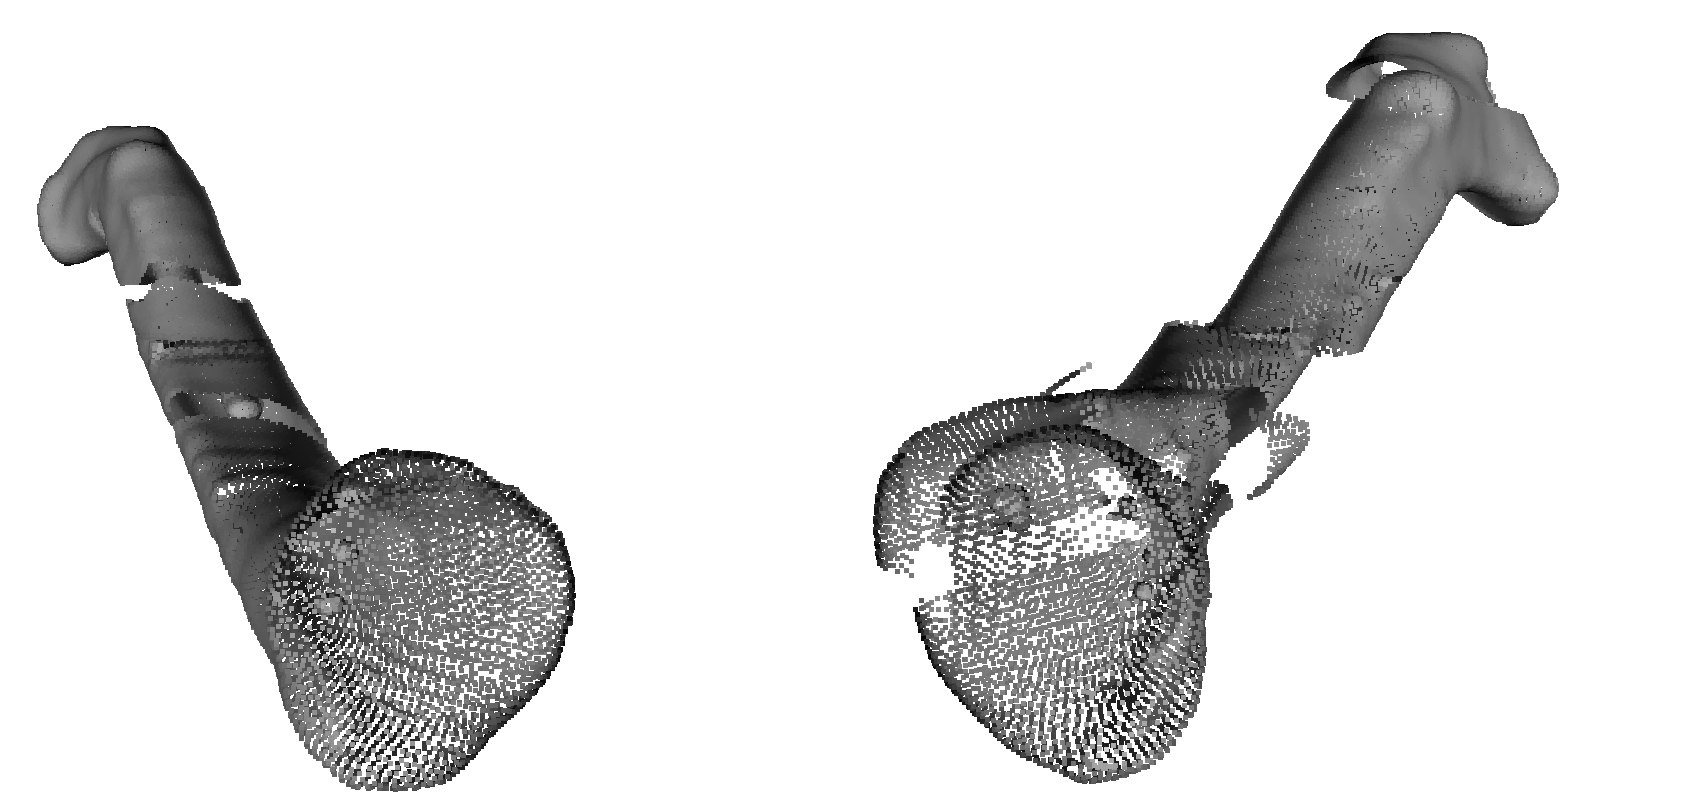
\includegraphics[width=.3\textwidth]{imagenes/chapter3/clavicula/clavicula_3.png}}
      \caption{Ejemplo de distorsiones generadas sobre clavículas, donde (a) es la imagen original, 
      (b) la distorsionada por submuestreo y (c) por movimiento local.}
      \label{fig:DistorsionesGeneradas}
    \end{figure}
  \vspace{-.3cm}
    \begin{enumerate}
      \item \textbf{11 nubes de puntos} de referencia.  
      \item \textbf{5} tipos de \textbf{distorsiones}: 
        submuestreo, compresión, ruido, rotación y movimiento local.
      \item \textbf{7 niveles} de intensidad para un \textbf{total de 385 nubes de puntos}.
    \end{enumerate}
\end{frame}

\begin{frame}
  \frametitle{Materiales: Generación de etiquetas}
  \begin{enumerate}
    \item Evitamos el problema logístico de obtención de la opinión media de calidad (MOS).
      \begin{itemize}
        \item Evaluación manual por grupo de personas en un entorno controlado.
      \end{itemize}
    \item Hacemos uso de las mejores métricas con referencia.
      \begin{itemize}
        \item Desglosamos el rendimiento por tipo de distorsión.
      \end{itemize}
  \end{enumerate}
\begin{table}
  \centering 
  \scriptsize
  \begin{tabular}{|c|c|c|}
    \hline
    \rowcolor[HTML]{FFC702}
     & \textbf{Parte I} & \textbf{Parte II} \\
    \hline 
    SROCC & 0.902697 & 0.878517\\
    \hline
    PLCC & 0.910713 & 0.871917\\
    \hline
  \end{tabular}
  \caption[Correlación de métricas sintéticas.]{
    Correlación de métricas sintéticas con experimento subjetivo de Liu et al\footnotemark[9].
}
  \label{tab:PseudoCorr}
\end{table}
\footnotetext[9]{\cite{ResSCNN}}
\end{frame}

\begin{frame}
  \frametitle{Métricas}
  \vspace{-.4cm}
  \begin{adjustwidth}{-.5cm}{}
  \begin{table}
      \setlength{\tabcolsep}{12pt}
  \begin{tabular}[l]{cc}
        \textbf{Correlación lineal de Pearson (PLCC)} 
        &
        \textbf{Correlación de rangos de Spearman (SROCC)} 
        \\
        \parbox[c]{6cm}{ 
   \centering
          $
  PLCC(x,y) = \frac{\sum_{i=1}^m (x_i - \bar x)(y_i - \bar y)}{\sqrt{\sum_{i=1}^m (x_i - \bar x)^2}\sqrt{\sum_{i=1}^m (y_i - \bar y)^2}}
        $ 
        \vspace{.3cm}
    }
& 
\parbox[c]{6cm}{
   \centering
   \vskip5pt
  $
  SROCC(x,y) = \frac{\sum_i (x_i - \bar x)(y_i - \bar y)}{\sqrt{\sum_i (x_i - \bar x)^2}\sqrt{\sum_i (y_i - \bar y)^2}}
        \vspace{.3cm}
$
}
\\ 
\parbox[c]{5cm}{
  \centering
  \footnotesize
    Evalúa si existe una \textbf{relación lineal} entre conjuntos. 
    \vspace{.5cm}
}
&
\parbox[c]{5cm}{
  \centering
  \footnotesize
  Evalúa la relación lineal entre los \textbf{\emph{rankings}}.
  \vspace{.5cm}
    \
}
\\
\parbox[c]{5cm}{\centering \textbf{Correlación de orden de rango de Kendall (KROCC)}}
& 
\textbf{Raíz del error cuadrático medio (RMSE)} 
\\
 \parbox[c]{5cm}{
   \centering
   \vskip5pt
   $
  KROCC(x,y) = \frac{C-D}{\frac{1}{2} m (m-1)}
    $
        \vspace{.3cm}
  }
& 
\parbox[c]{5cm}{
  \centering
  $
  RMSE(x,y) = \sqrt{\frac{1}{m}\sum_{i=1}^m (x_i - y_i)^2}
  $
}
\\
\parbox[c]{5cm}{
  \centering
  \footnotesize
    Evalúa la \textbf{concordancia y discordancia} de relación entre pares.
  }
  & 
\parbox[c]{5cm}{
  \centering
  \footnotesize
  Evalúa la \textbf{diferencia media} de los pares de valores.
   
  }
  \\

      \end{tabular}
  \end{table}
\end{adjustwidth} 
\end{frame}


\subsection{Métodos}
\begin{frame}
  \frametitle{Modelo NR3DQA\footnote[frame]{\cite{NR3DQA}}}
  \begin{columns}
    \column{0.5\textwidth}
    \begin{enumerate}
      \item \textbf{Extracción independiente} del modelo.
        \begin{itemize}
          \item Anisotropía
          \item Planaridad
          \item Esfericidad 
          \item Curvatura 
          \item Linealidad
        \end{itemize}
      \item \textbf{Descartamos} las características lumínicas.
      \item Usamos: \textbf{media, desviación y entropía}.
    \end{enumerate}
    \column{0.5\textwidth}
    \begin{figure}
      \begin{center}
        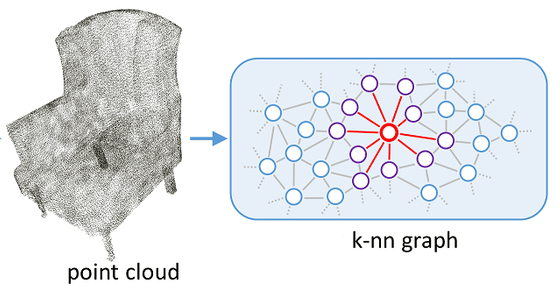
\includegraphics[width=\textwidth]{imagenes/chapter3/PatchSelection}
      \end{center}
      \caption{Extracción de características del vecindario.}
    \end{figure}
    \end{columns}
\end{frame}

\begin{frame}
  \frametitle{Modelo VQA-PC\footnote[frame]{\cite{VQA-PC}}}
  \begin{columns}
    \column{0.5\textwidth}
    \begin{enumerate}
      \item \textbf{Extracción automática} de características.
      \item Extracción \textbf{espacial y temporal} de las reconstrucciones.
        \begin{itemize}
          \item Espacial por fotogramas estáticos de \textbf{distintas perspectivas}.
          \item Temporal por tratar la \textbf{nube como video}.
        \end{itemize}
      \item Es como un \textbf{meta-modelo} de aprendizaje profundo. 
    \end{enumerate}
    \column{0.5\textwidth}
    \begin{figure}
      \begin{center}
        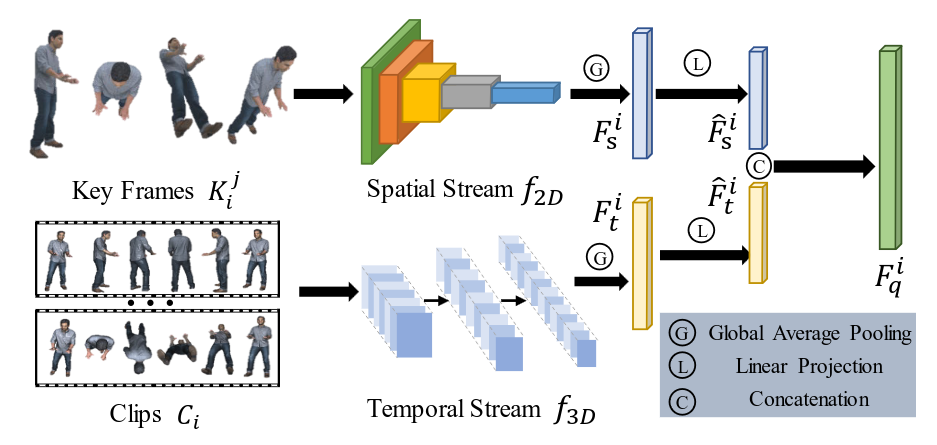
\includegraphics[width=\textwidth]{imagenes/chapter3/PipelineCompleto}
      \end{center}
      \caption{Estructura del modelo VQA-PC\footnotemark[11]}
    \end{figure}
  \end{columns}
\end{frame}

\subsection{Entorno}
\begin{frame}
  \frametitle{Tecnologías utilizadas}
  \begin{table}[htp]
    \vspace{-.5cm}
      \begin{tabular}{cccc}
        \begin{minipage}{.2\textwidth}
          
\includegraphics[width=\textwidth]{imagenes/chapter3/Python}
        \end{minipage} 
                                  & 
        \begin{minipage}{.2\textwidth}
          
\includegraphics[width=.9\textwidth]{imagenes/chapter3/FastAI}
        \end{minipage} 
                                  & 
        \begin{minipage}{.2\textwidth}
          
\includegraphics[width=\textwidth]{imagenes/chapter3/Pytorch}
        \end{minipage} 
                                  &
        \begin{minipage}{.2\textwidth}
          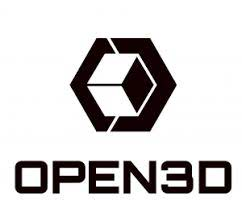
\includegraphics[width=.9\textwidth]{imagenes/chapter3/Open3D}
        \end{minipage} 
                                  \\
        \begin{minipage}{.2\textwidth}
          
\includegraphics[width=\textwidth]{imagenes/chapter3/Numpy}
        \end{minipage} 
                                                        & 
        \begin{minipage}{.2\textwidth}
          
\includegraphics[width=.9\textwidth]{imagenes/chapter3/Scikit}
        \end{minipage} 
                                                        & 
        \begin{minipage}{.2\textwidth}
          
\includegraphics[width=.9\textwidth]{imagenes/chapter3/Polars}
        \end{minipage} 
        &
                                                        \\
                                                        & 
        \begin{minipage}{.2\textwidth}
          
\includegraphics[width=.9\textwidth]{imagenes/chapter3/Nvidia}
        \end{minipage} 
                                                        & 
        \begin{minipage}{.2\textwidth}
          
\includegraphics[width=.9\textwidth]{imagenes/chapter3/Colab}
        \end{minipage} 
                                                        &
                                                        \\
      \end{tabular}
  \end{table}
\end{frame}
